\documentclass[a4paper,11pt,fleqn]{scrartcl}
\usepackage[german,ngerman]{babel}
\usepackage[utf8]{inputenc}
\usepackage[T1]{fontenc}
\usepackage[top=1.3in, bottom=1.2in, left=0.9in, right=0.9in]{geometry}
\usepackage{lmodern}
\usepackage{amssymb}
\usepackage{amsmath}
\usepackage{enumerate}
\usepackage{fancyhdr}
\usepackage{color}
\usepackage{tikz}

% ------------------------------------------------------

% Commands

\newcommand{\todo}{\textcolor{red}{\textbf{TODO}}}
\newcommand{\authorinfo}{Arne Struck, Jonathan Werner}
\newcommand{\titleinfo}{HLR OPENMP, Blatt 4}
\newcommand{\qed}{\ \square}


% ------------------------------------------------------

% Title & Pages

\title{\titleinfo}
\author{\authorinfo}

\pagestyle{fancy}
\fancyhf{}
\fancyhead[L]{\authorinfo}
\fancyhead[R]{\titleinfo}
\fancyfoot[C]{\thepage}

\begin{document}
\maketitle
\notag


\section{Optimierung}\label{optimierung}

\textbf{Sequentiell, ohne \texttt{-fopenmp}:}

\texttt{./partdiff-seq 1 2 512 2 2 200} braucht \textbf{120.29s}.

\textbf{1 Thread, mit \texttt{-fopenmp}:}

\texttt{./partdiff-seq 1 2 512 2 2 200} braucht \textbf{120.65s}.

\textbf{12 Threads, mit \texttt{-fopenmp}:}

\texttt{./partdiff-seq 1 2 512 2 2 200} braucht \textbf{14.9s}.

\textbf{Mit verschiedenen Schedulings, jw 12 Threads:}

\begin{itemize}
\itemsep1pt\parskip0pt\parsep0pt
\item
  \textbf{\texttt{schedule(dynamic, 1)}:}

  \begin{itemize}
  \itemsep1pt\parskip0pt\parsep0pt
  \item
    \texttt{./partdiff-seq 1 2 512 2 2 200} braucht \textbf{11.39s}.
  \item
    Speedup zu ohne OMP: \textbf{10.59}. The winner! :)
  \end{itemize}
\item
  \textbf{\texttt{schedule(dynamic, 4)}:}

  \begin{itemize}
  \itemsep1pt\parskip0pt\parsep0pt
  \item
    \texttt{./partdiff-seq 1 2 512 2 2 200} braucht \textbf{14.2s}.
  \item
    Speedup zu ohne OMP: \textbf{\textasciitilde{}8.5}.
  \end{itemize}
\item
  \textbf{\texttt{schedule(guided)}:}

  \begin{itemize}
  \itemsep1pt\parskip0pt\parsep0pt
  \item
    \texttt{./partdiff-seq 1 2 512 2 2 200} braucht \textbf{12.3s}.
  \item
    Speedup zu ohne OMP: \textbf{9.8}.
  \end{itemize}
\item
  \textbf{\texttt{schedule(static, 1)}:}

  \begin{itemize}
  \itemsep1pt\parskip0pt\parsep0pt
  \item
    \texttt{./partdiff-seq 1 2 512 2 2 200} braucht \textbf{14.1s}.
  \end{itemize}
\item
  \textbf{\texttt{schedule(static, 2)}:}

  \begin{itemize}
  \itemsep1pt\parskip0pt\parsep0pt
  \item
    \texttt{./partdiff-seq 1 2 512 2 2 200} braucht \textbf{14.7s}.
  \end{itemize}
\item
  \textbf{\texttt{schedule(static, 16)}:}

  \begin{itemize}
  \itemsep1pt\parskip0pt\parsep0pt
  \item
    \texttt{./partdiff-seq 1 2 512 2 2 200} braucht \textbf{14.57s}.
  \end{itemize}
\end{itemize}

Zeit benötigt: 2h. Fehlersuche? Ja, zuerst haben wir die simple
interference function geenommen und dadurch nur ein Speedup von 4
erreicht.


\newpage
\section{Messungen}\label{messungen}

\subsection{Messung 1}\label{messung-1}
\begin{center}
\begin{tabular}[c]{l|l|l}
procs & speedup & time in sec \\ \hline

1 (no OMP) & 1 & 120.29 \\
1 & 1 & 120.65 \\
2 & 2.044222298 & 59.02 \\
3 & 2.960009814 & 40.76 \\
4 & 4.045942321 & 29.82 \\
5 & 4.868845843 & 24.78 \\ 
6 & 5.952146029 & 20.27 \\
7 & 6.710233593 & 17.98 \\
8 & 7.65060241 & 15.77 \\
9 & 8.431167016 & 14.31 \\
10 & 9.1332324 & 13.21 \\
11 & 9.913722268 & 12.17 \\
12 & 9.995857498 & 12.07 \\
\end{tabular}

\end{center}

\begin{figure}[htbp]
\centering
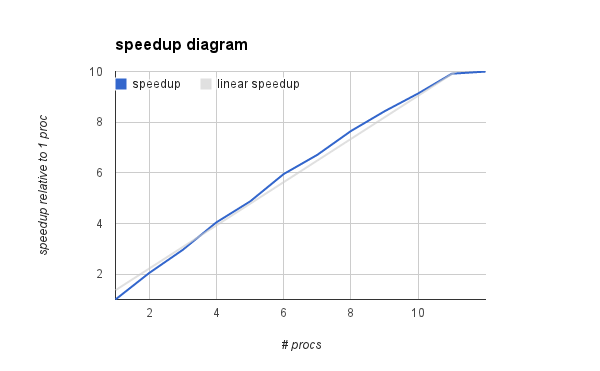
\includegraphics[scale=0.8]{speedup.png}
\caption{}
\end{figure}

\end{document}